%\title{LaTeX Portrait Poster Template}
%%%%%%%%%%%%%%%%%%%%%%%%%%%%%%%%%%%%%%%%%
% a0poster Portrait Poster
% LaTeX Template
% Version 1.0 (22/06/13)
%
% The a0poster class was created by:
% Gerlinde Kettl and Matthias Weiser (tex@kettl.de)
% 
% This template has been downloaded from:
% http://www.LaTeXTemplates.com
%
% License:
% CC BY-NC-SA 3.0 (http://creativecommons.org/licenses/by-nc-sa/3.0/)
%
%%%%%%%%%%%%%%%%%%%%%%%%%%%%%%%%%%%%%%%%%

%----------------------------------------------------------------------------------------
%	PACKAGES AND OTHER DOCUMENT CONFIGURATIONS
%----------------------------------------------------------------------------------------

\documentclass[a0,portrait]{a0poster}

\usepackage{multicol} % This is so we can have multiple columns of text side-by-side
\columnsep=100pt % This is the amount of white space between the columns in the poster
\columnseprule=3pt % This is the thickness of the black line between the columns in the poster

\usepackage[svgnames]{xcolor} % Specify colors by their 'svgnames', for a full list of all colors available see here: http://www.latextemplates.com/svgnames-colors

\usepackage{times} % Use the times font
%\usepackage{palatino} % Uncomment to use the Palatino font

\usepackage{graphicx} % Required for including images
\graphicspath{{figures/}} % Location of the graphics files
\usepackage{booktabs} % Top and bottom rules for table
\usepackage[font=small,labelfont=bf]{caption} % Required for specifying captions to tables and figures
\usepackage{amsfonts, amsmath, amsthm, amssymb} % For math fonts, symbols and environments
\usepackage{wrapfig} % Allows wrapping text around tables and figures

\usepackage{listings}
\usepackage{sectsty}

\sectionfont{\LARGE}
\begin{document}

%----------------------------------------------------------------------------------------
%	POSTER HEADER 
%----------------------------------------------------------------------------------------

% The header is divided into two boxes:
% The first is 75% wide and houses the title, subtitle, names, university/organization and contact information
% The second is 25% wide and houses a logo for your university/organization or a photo of you
% The widths of these boxes can be easily edited to accommodate your content as you see fit
\begin{minipage}[b]{0.15\linewidth}

\includegraphics[width=11cm]{iyte_logo.png}
\end{minipage}
\hspace{1.5cm}
\begin{minipage}[b]{0.70\linewidth}
\Huge \color{DarkRed} \textbf{RAPPROX - Resource-Aware Compiler Design for \\ Approximate Computing Techniques in GPGPUs} \color{Black}\\ \\% Title
%\Huge\textit{An Exploration of Complexity}\\[2cm] % Subtitle
\huge \textbf{PARS Research Group}\\[0.5cm] % Author(s)
\huge Computer Engineering Department, Izmir Institute of Technology\\[0.4cm] % University/organization
\Large \texttt{https://parsiyte.github.io/} \\
\end{minipage}
%
\begin{minipage}[b]{0.15\linewidth}

\includegraphics[width=12cm]{pars.png}%
\includegraphics[width=5cm]{pars_qr.png}\\
\end{minipage}

\vspace{1cm} % A bit of extra whitespace between the header and poster content

%----------------------------------------------------------------------------------------

\begin{multicols}{2} % This is how many columns your poster will be broken into, a portrait poster is generally split into 2 columns


%----------------------------------------------------------------------------------------
%	ABSTRACT
%----------------------------------------------------------------------------------------

\color{Navy} % Navy color for the abstract

%----------------------------------------------------------------------------------------
%	INTRODUCTION
%----------------------------------------------------------------------------------------

\color{SaddleBrown} % SaddleBrown color for the introduction

\section*{Work Description}
\Large
Novel approximate computing techniques by considering architecture-specific features of
GPUs and develop a compiler framework to perform those techniques automatically for the target CUDA program

\noindent Optimum Pareto solutions using a systematic design
space exploration methodology to choose the approximate computing techniques

\noindent Parallel metaheuristics techniques which generate better results in reasonable times by considering energy consumption, performance, and accuracy rates of the approximate CUDA
programs

%Our compiler framework generates approximate source codes by considering performance and energy resources. Our parallel metaheuristic algorithm solves the multi-objective optimization problem by utilizing the parallel resources of the underlying multicore system efficiently. We execute CUDA program versions that implement different approximation techniques simultaneously in multi-GPUs available in the system and shorten the performance evaluation phase. Our compiler generates executable files, including optimum pareto solutions, by executing our metaheuristic algorithm, which includes problem-specific operators to escape from local optimum or infeasible solutions. 
\normalsize
\begin{center}\vspace{1cm}
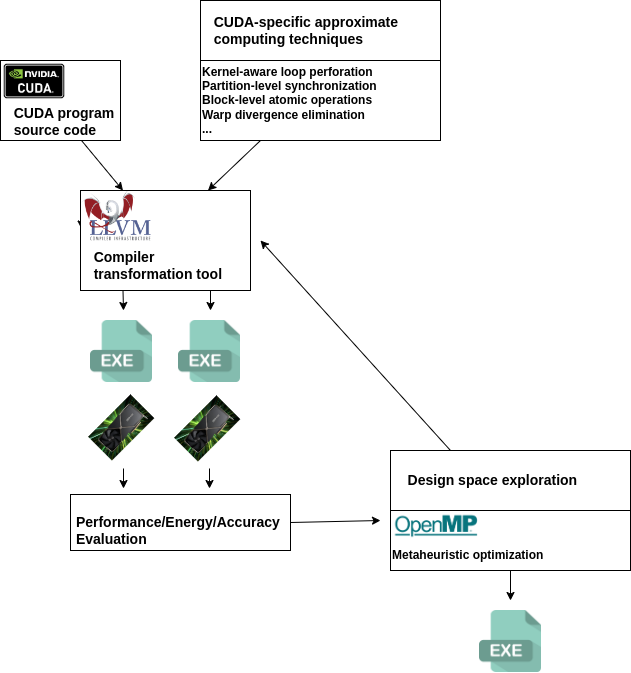
\includegraphics[width=0.8\linewidth]{RAPPROX.png}
%\captionof{figure}{\color{Green} Figure caption}
\end{center}\vspace{0.5cm}

%----------------------------------------------------------------------------------------
%	OBJECTIVES
%----------------------------------------------------------------------------------------

\color{DarkSlateGray} % DarkSlateGray color for the rest of the content

\section*{Main Objectives}
\Large
\begin{enumerate}
\item Approximate computation methods specific to GPU architectures considering GPGPU applications
\item Developing a compiler tool applying the developed approximate computation methods
\item Evaluation of the performance, energy, and accuracy values by running candidate program versions 
\item Metaheuristic method that performs design space exploration by evaluating the approximate calculation methods and different parameters 
\end{enumerate}
\normalsize
%----------------------------------------------------------------------------------------
%	MATERIALS AND METHODS
%----------------------------------------------------------------------------------------

\section*{Approximation for CUDA Programs}
\Large
\begin{enumerate}
\item Kernel-aware loop perforation
\begin{itemize}
    \item Kernel launch perforation
    \item Kernel launch configuration perforation
    \item Intra-kernel loop perforation
\end{itemize}
\item Relaxed synchronization
\begin{itemize}
    \item Partition-level synchronization
    \item Block-level atomic operations
\end{itemize}
\item Warp divergence elimination
\end{enumerate}
\normalsize



%------------------------------------------------


%	RESULTS 
%----------------------------------------------------------------------------------------
\section*{Source-to-Source Compiler Transformation} 
\begin{center}\vspace{1cm}
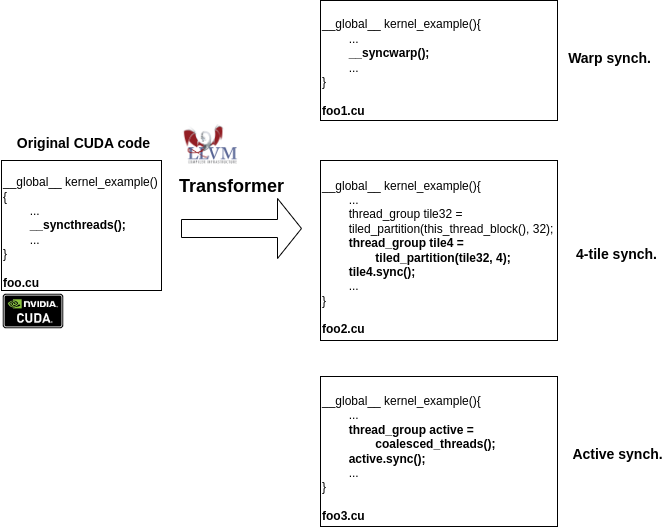
\includegraphics[width=0.8\linewidth]{figures/Source-to-Source.drawio.png}
%\captionof{figure}{\color{Green} Figure caption}
\end{center}\vspace{1cm}

\section*{Design Space Exploration}
\Large
\begin{itemize}
    \item Multiobjective optimization
\begin{itemize}
    \item High performance
    \item Low energy consumption
    \item Acceptable accuracy
\end{itemize}
\item Solution representation for target programs
\item Problem-specific variation operators
\end{itemize}
\normalsize

\section*{Preliminary Results}

\begin{center}\vspace{1cm}
{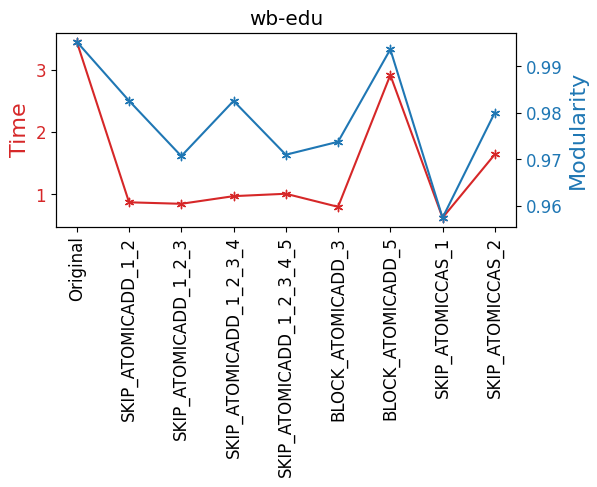
\includegraphics[width=.48\columnwidth]{web-edu.png}\label{fig:wb-edu}}
%{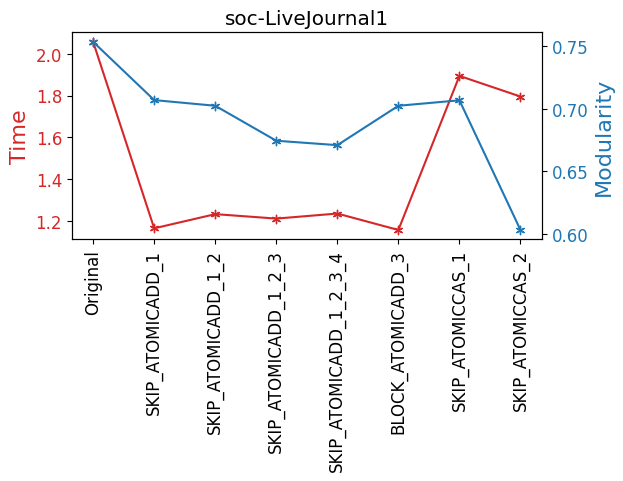
\includegraphics[width=.55\columnwidth]{socLiveJournal.png}\label{fig:socLiveJournal}}
{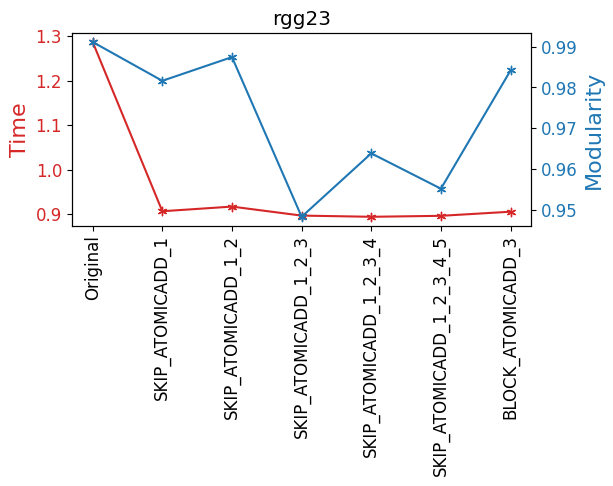
\includegraphics[width=.48\columnwidth]{rgg23.png}\label{fig:rgg23}}
{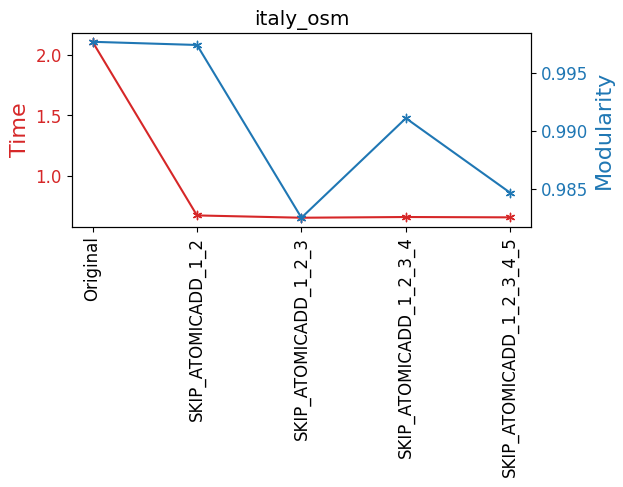
\includegraphics[width=.48\columnwidth]{italy_osm.png}\label{fig:italy}}
{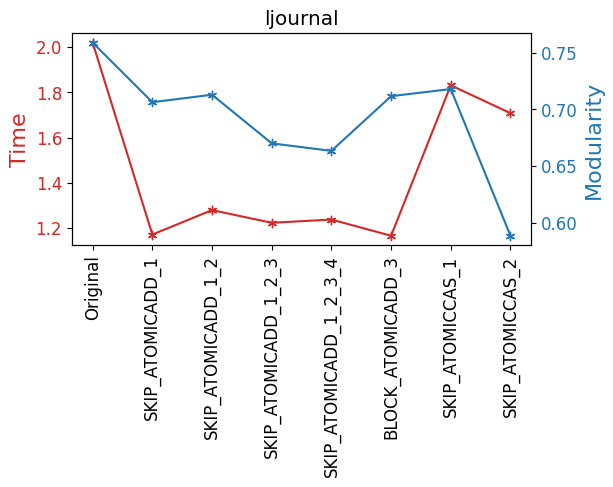
\includegraphics[width=.48\columnwidth]{ljournal.png}\label{fig:ljournal}}
\end{center}\vspace{1cm}





%----------------------------------------------------------------------------------------
%	CONCLUSIONS
%----------------------------------------------------------------------------------------

\color{SaddleBrown} % SaddleBrown color for the conclusions to make them stand out



\color{DarkSlateGray} % Set the color back to DarkSlateGray for the rest of the content

%----------------------------------------------------------------------------------------
%	FORTHCOMING RESEARCH
%----------------------------------------------------------------------------------------

%----------------------------------------------------------------------------------------
%	REFERENCES
%----------------------------------------------------------------------------------------

\nocite{*} % Print all references regardless of whether they were cited in the poster or not
\bibliographystyle{plain} % Plain referencing style
\bibliography{sample} % Use the example bibliography file sample.bib

%----------------------------------------------------------------------------------------
%	ACKNOWLEDGEMENTS
%----------------------------------------------------------------------------------------

\section*{Acknowledgements}

This work was supported by the Scientific and Technological Research Council of Turkey (TÜBİTAK), Grant No: 122E395. This work is partially supported by CERCIRAS COST Action CA19135 funded by COST Association.

%----------------------------------------------------------------------------------------

\end{multicols}
\end{document}